% !TeX root = main.tex
\section*{Results and discussion}
To find a good optimum for the exposure time, the checkerboard pattern is compared for each sample. Microscope images of the samples with positive  and with exposure times coming close\footnote{Images of the checkerboard pattern for all samples can be found in the appendix.}to an optimum are compared below in figure \ref{fig:b3d1},\ref{fig:b3a1} and \ref{fig:b3e1}:

\begin{figure}[H]
	\centering
	\resizebox{\linewidth}{!}{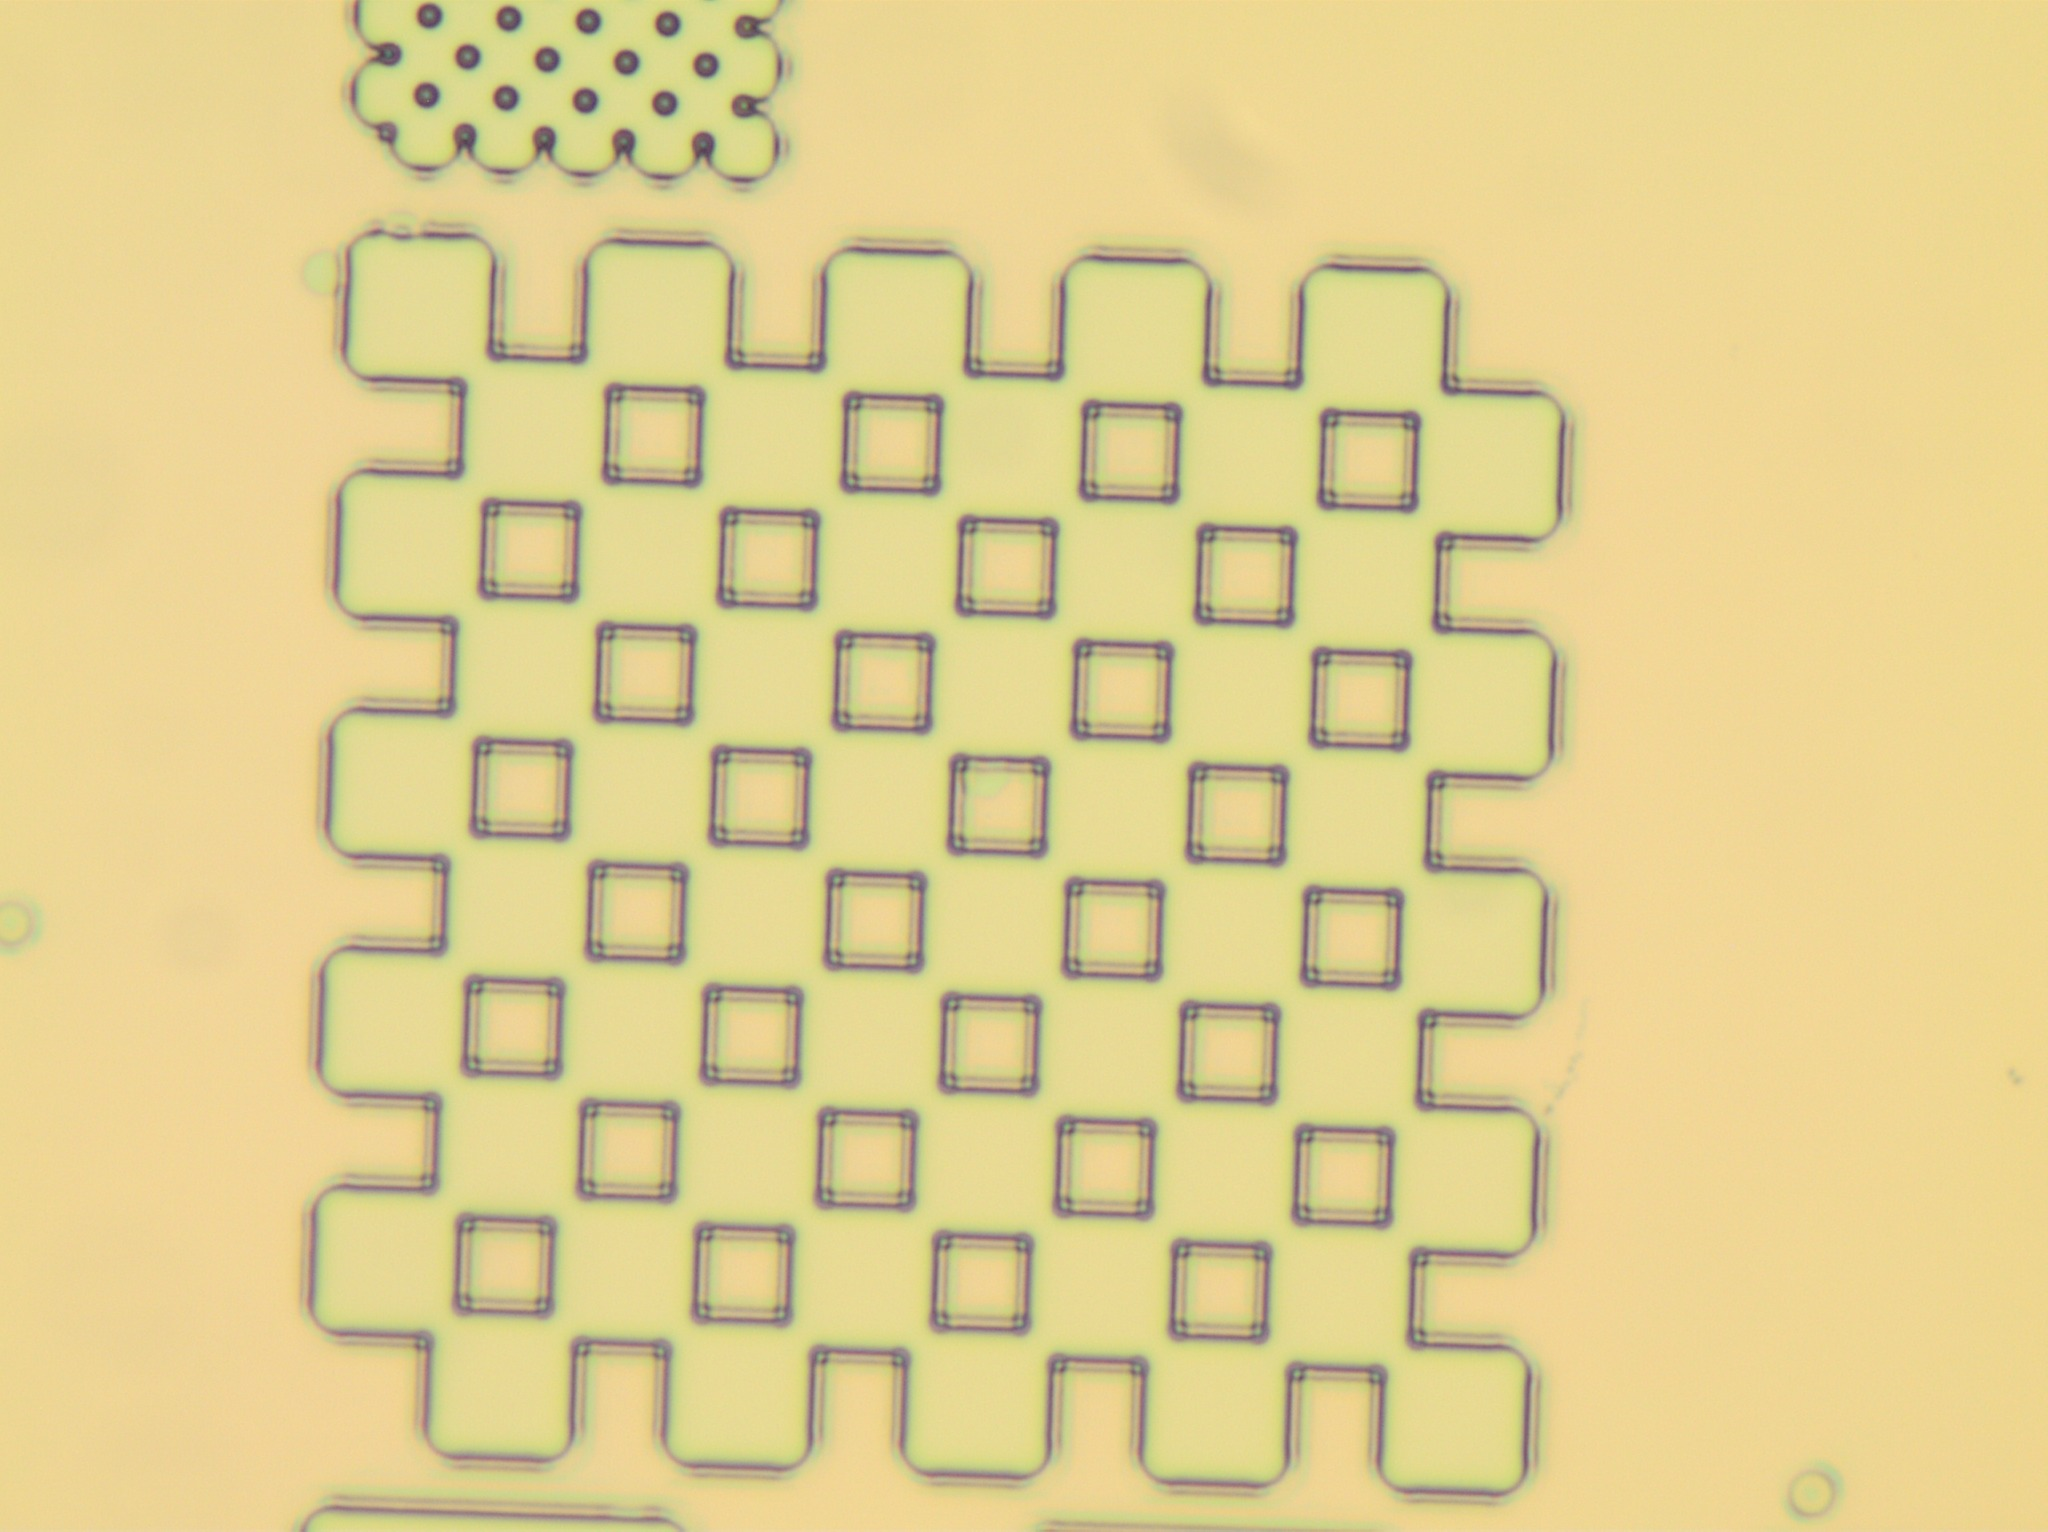
\includegraphics{data/b3d1.jpg}}
	\caption{Sample is exposed for 1 minute. Significant underexposure can be seen.}
	\label{fig:b3d1}
\end{figure}
\begin{figure}[H]
	\centering
	\resizebox{\linewidth}{!}{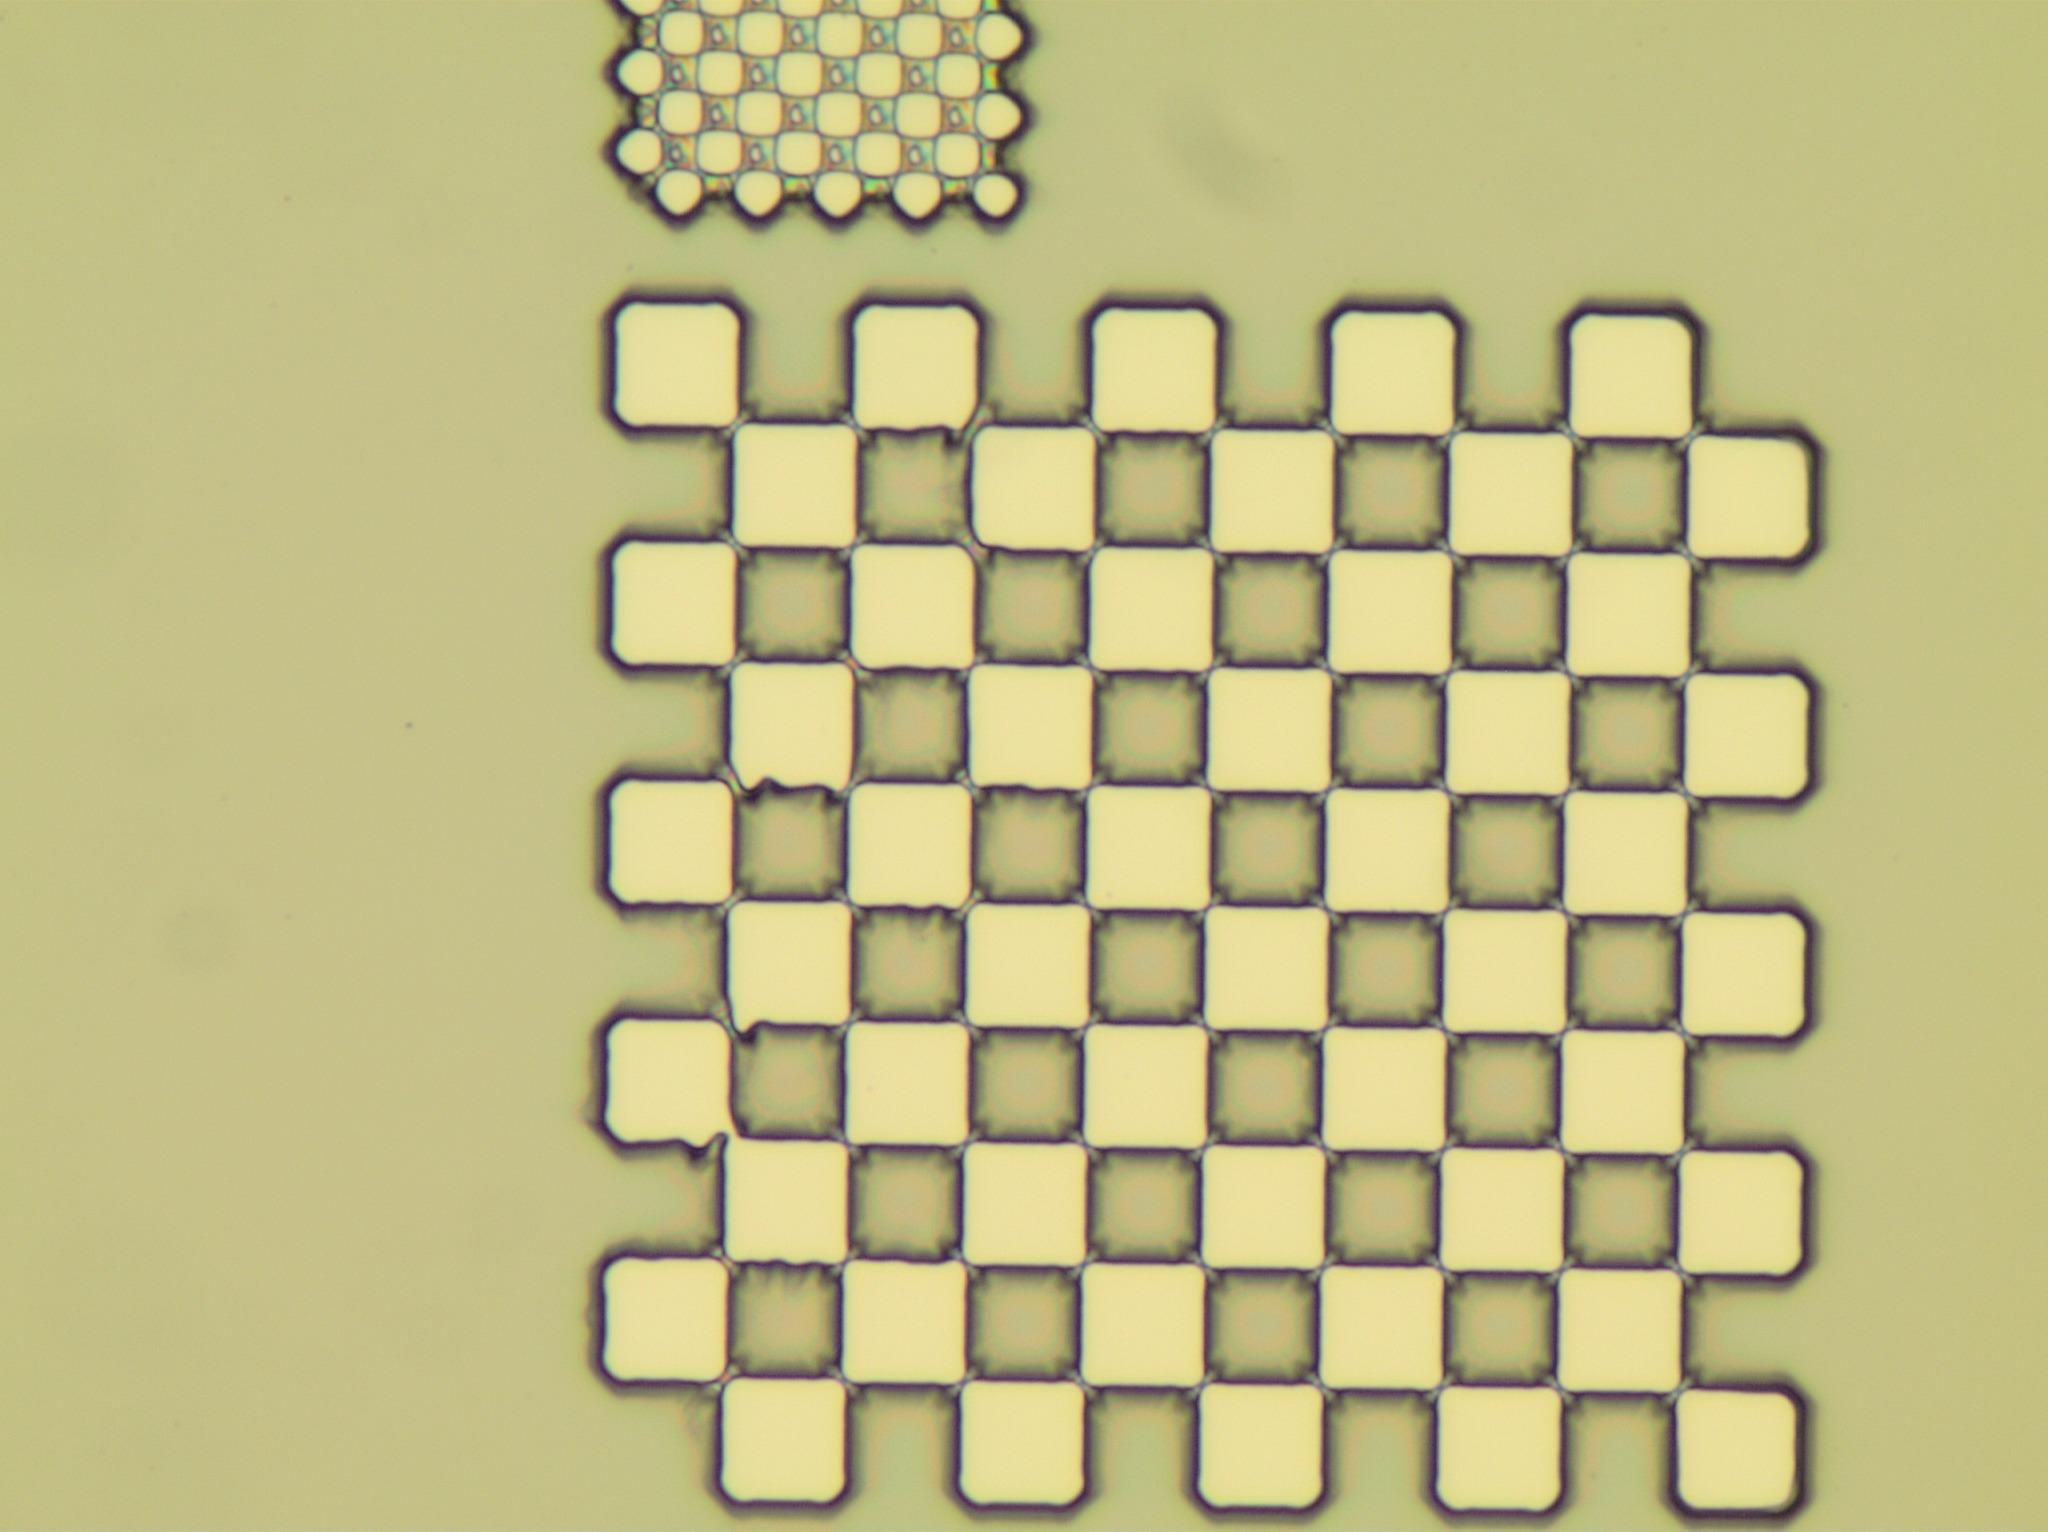
\includegraphics{data/b3e1.jpg}}
	\caption{Sample is exposed for 2.5 minutes. Slight overexposure can be seen at the vertices of the squares.}
	\label{fig:b3e1}
\end{figure}
\begin{figure}[H]
	\centering
	\resizebox{\linewidth}{!}{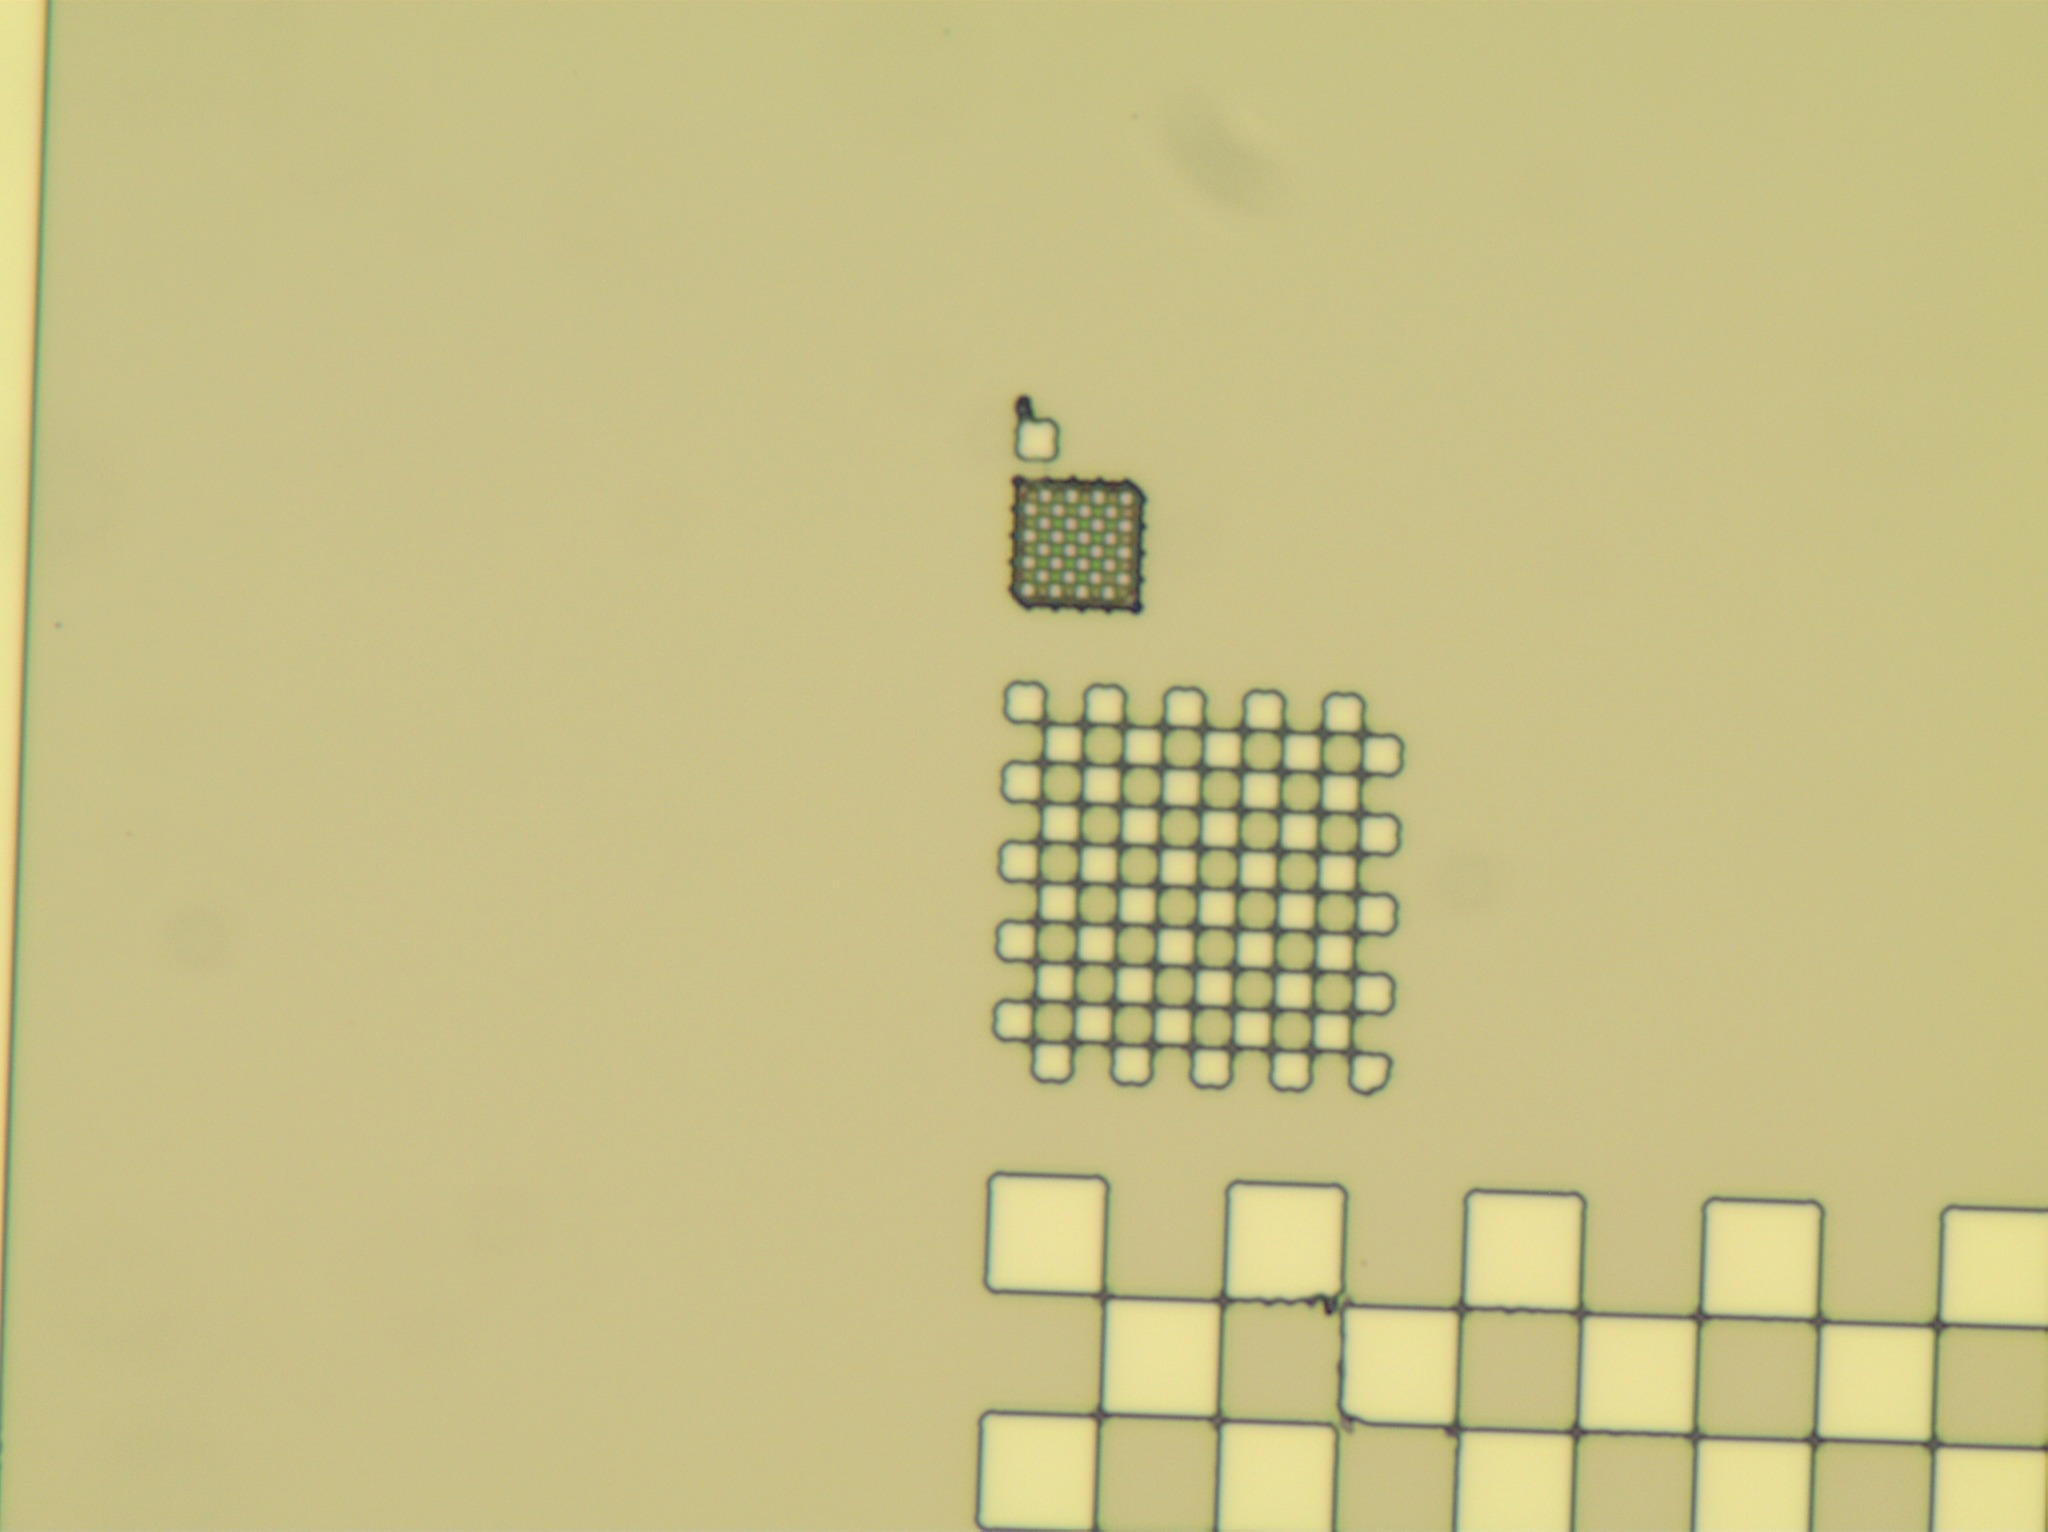
\includegraphics{data/b3a1.jpg}}
	\caption{Sample is exposed for 2 minutes. Note that the checkerboard pattern in the lower-right corner is of the same size as the one in the previous figures.}
	\label{fig:b3a1}
\end{figure}

With the limited amount of developed samples, an exposure time of 2 minutes was found to be optimal. Several images taken with a Hitachi S4800 scanning electron microscope are shown in figures \ref{fig:b2d4_q4}-\ref{fig:b2d10_q11}:

%\begin{figure}[H]
%	\centering
%	\resizebox{\linewidth}{!}{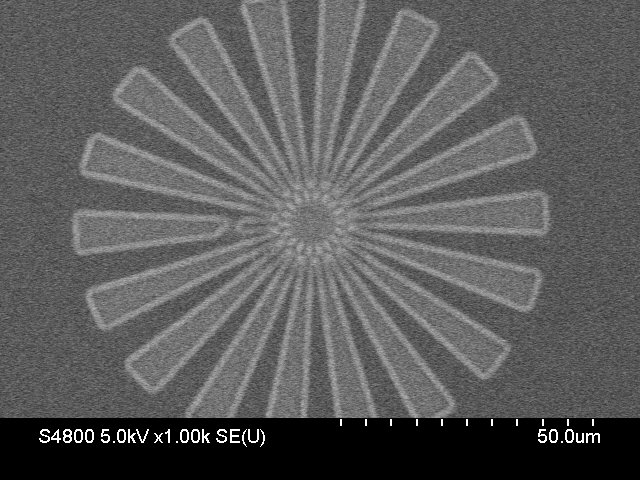
\includegraphics{data/sem/b3a1_q01.jpg}}
%	\caption{SEM}
%	\label{fig:b2d1_q1}
%\end{figure}
%\begin{figure}[H]
%	\centering
%	\resizebox{\linewidth}{!}{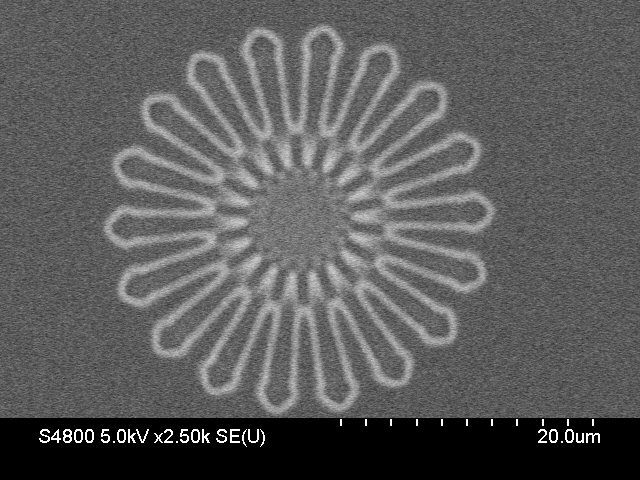
\includegraphics{data/sem/b3a2_q02.jpg}}
%	\caption{SEM}
%	\label{fig:b2d2_q2}
%\end{figure}
%\begin{figure}[H]
%	\centering
%	\resizebox{\linewidth}{!}{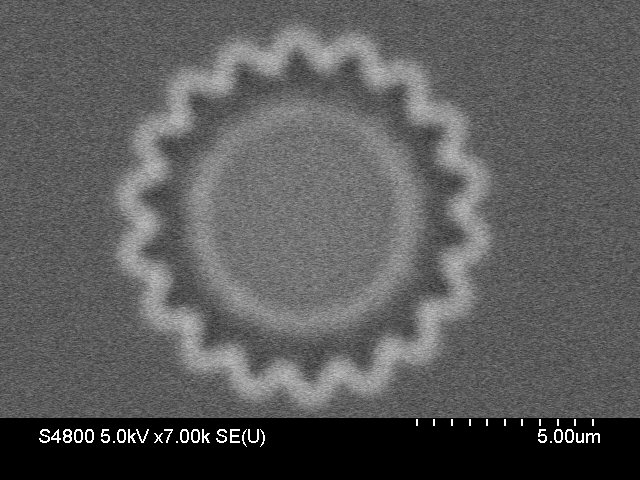
\includegraphics{data/sem/b3a3_q03.jpg}}
%	\caption{SEM}
%	\label{fig:b2d3_q3}
%\end{figure}
\begin{figure}[H]
	\centering
	\resizebox{\linewidth}{!}{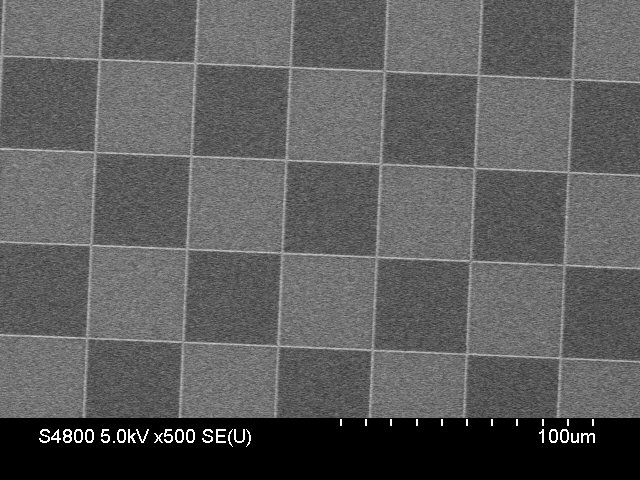
\includegraphics{data/sem/b3a4_q04.jpg}}
	\caption{Structure size of $\sim$32 $\mu$m.}
	\label{fig:b2d4_q4}
\end{figure}
\begin{figure}[H]
	\centering
	\resizebox{\linewidth}{!}{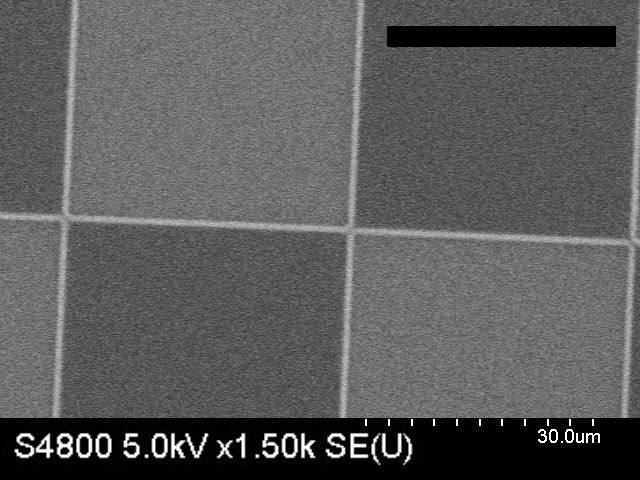
\includegraphics{data/sem/b3a5_q05.jpg}}
	\caption{Zoom in on the checkerboard pattern with structure size of $\sim$35}
	\label{fig:b2d5_q5}
\end{figure}
\begin{figure}[H]
	\centering
	\resizebox{\linewidth}{!}{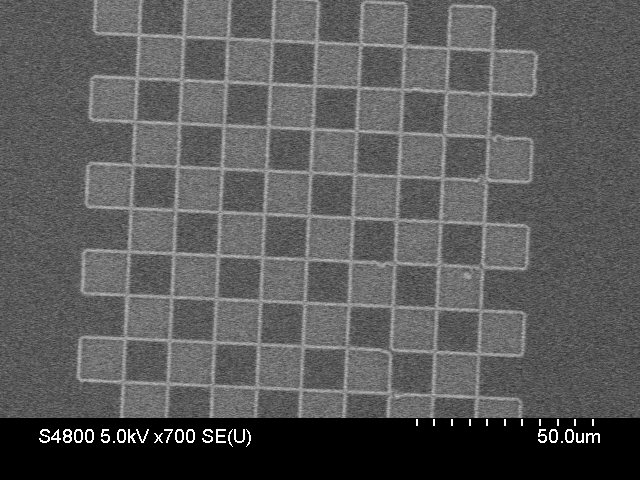
\includegraphics{data/sem/b3a6_q06.jpg}}
	\caption{Structure size of $\sim$10 $\mu$m.}
	\label{fig:b2d6_q6}
\end{figure}
\begin{figure}[H]
	\centering
	\resizebox{\linewidth}{!}{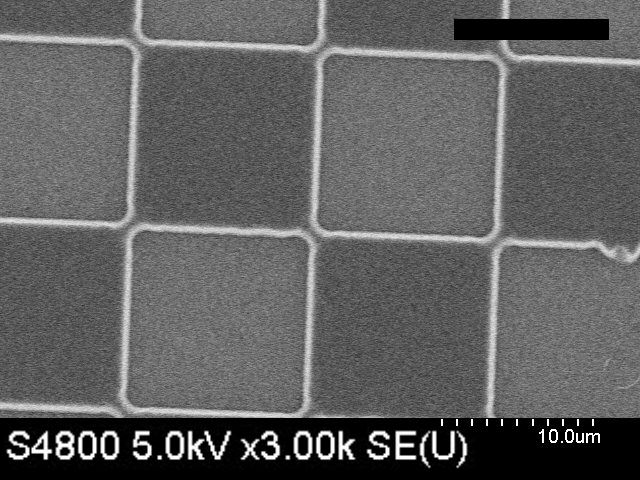
\includegraphics{data/sem/b3a7_q07.jpg}}
	\caption{Zoom in on the checkerboard pattern with structure size of $\sim$10 $\mu$m. Slight overexposure can be seen at the vertices of the squares.}
	\label{fig:b2d7_q7}
\end{figure}
\begin{figure}[H]
	\centering
	\resizebox{\linewidth}{!}{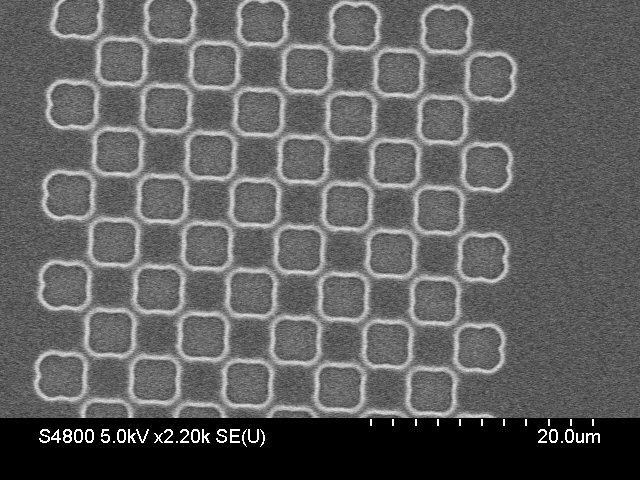
\includegraphics{data/sem/b3a8_q08.jpg}}
	\caption{Structure size of $\sim$3 $\mu$m.}
	\label{fig:b2d8_q8}
\end{figure}
\begin{figure}[H]
	\centering
	\resizebox{\linewidth}{!}{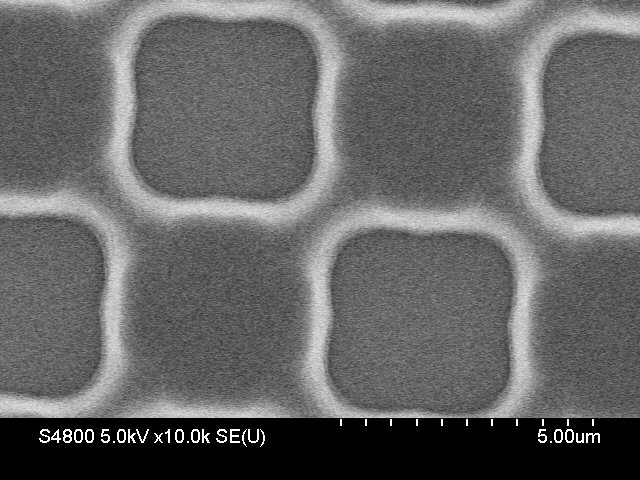
\includegraphics{data/sem/b3a9_q09.jpg}}
	\caption{Zoom in on the checkerboard pattern with structure size of $\sim$3 $\mu$m. The effects of overexposure become pronounced at structure sizes of $\sim$3 $\mu$m.}
	\label{fig:b2d9_q9}
\end{figure}
\begin{figure}[H]
	\centering
	\resizebox{\linewidth}{!}{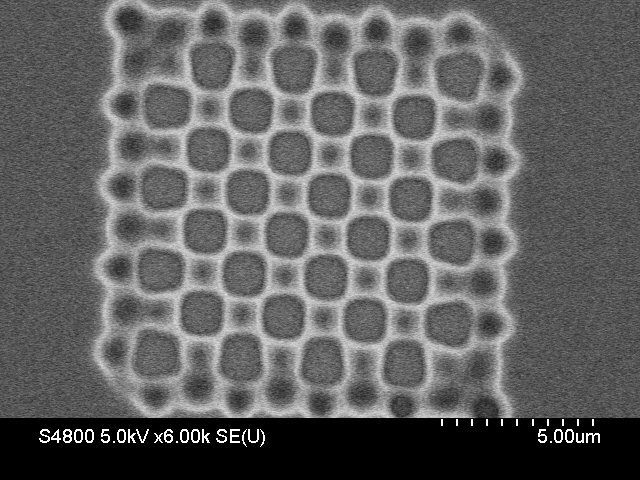
\includegraphics{data/sem/b3a10_q10.jpg}}
	\caption{SEM}
	\label{fig:b2d10_q10}
\end{figure}
\begin{figure}[H]
	\centering
	\resizebox{\linewidth}{!}{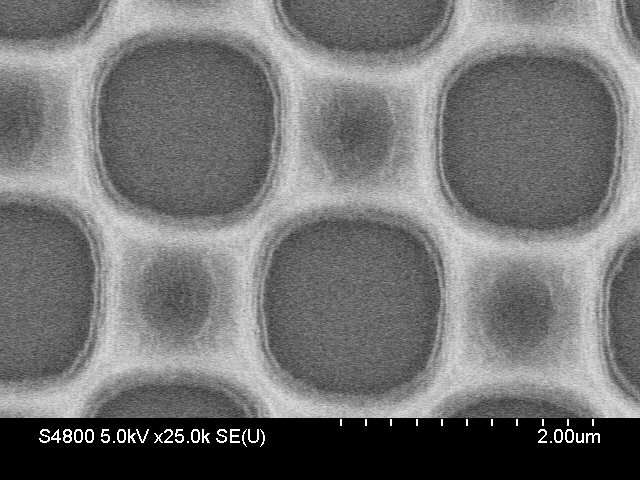
\includegraphics{data/sem/b3a10_q11.jpg}}
	\caption{SEM}
	\label{fig:b2d10_q11}
\end{figure}

The checkerboard pattern starts to decline in resolution between lengths of 2 and 10 $\mu$m. The images taken with the SEM show the same decline in resolution between 2 and 10 $\mu$m, as can be seen in the appendix.


It was found that for the negative recipe an exposure time of 0.1 minute resulted in no pattern creation at all, while exposure times of 0.5 minutes and longer resulted in overexposure of the pattern. The results of the developed samples with exposure times between 0.1 and 0.5 minutes are shown in figures \ref{fig:b2d1}, \ref{fig:b2h1} and \ref{fig:b2i1}:

\begin{figure}[H]
	\centering
	\resizebox{\linewidth}{!}{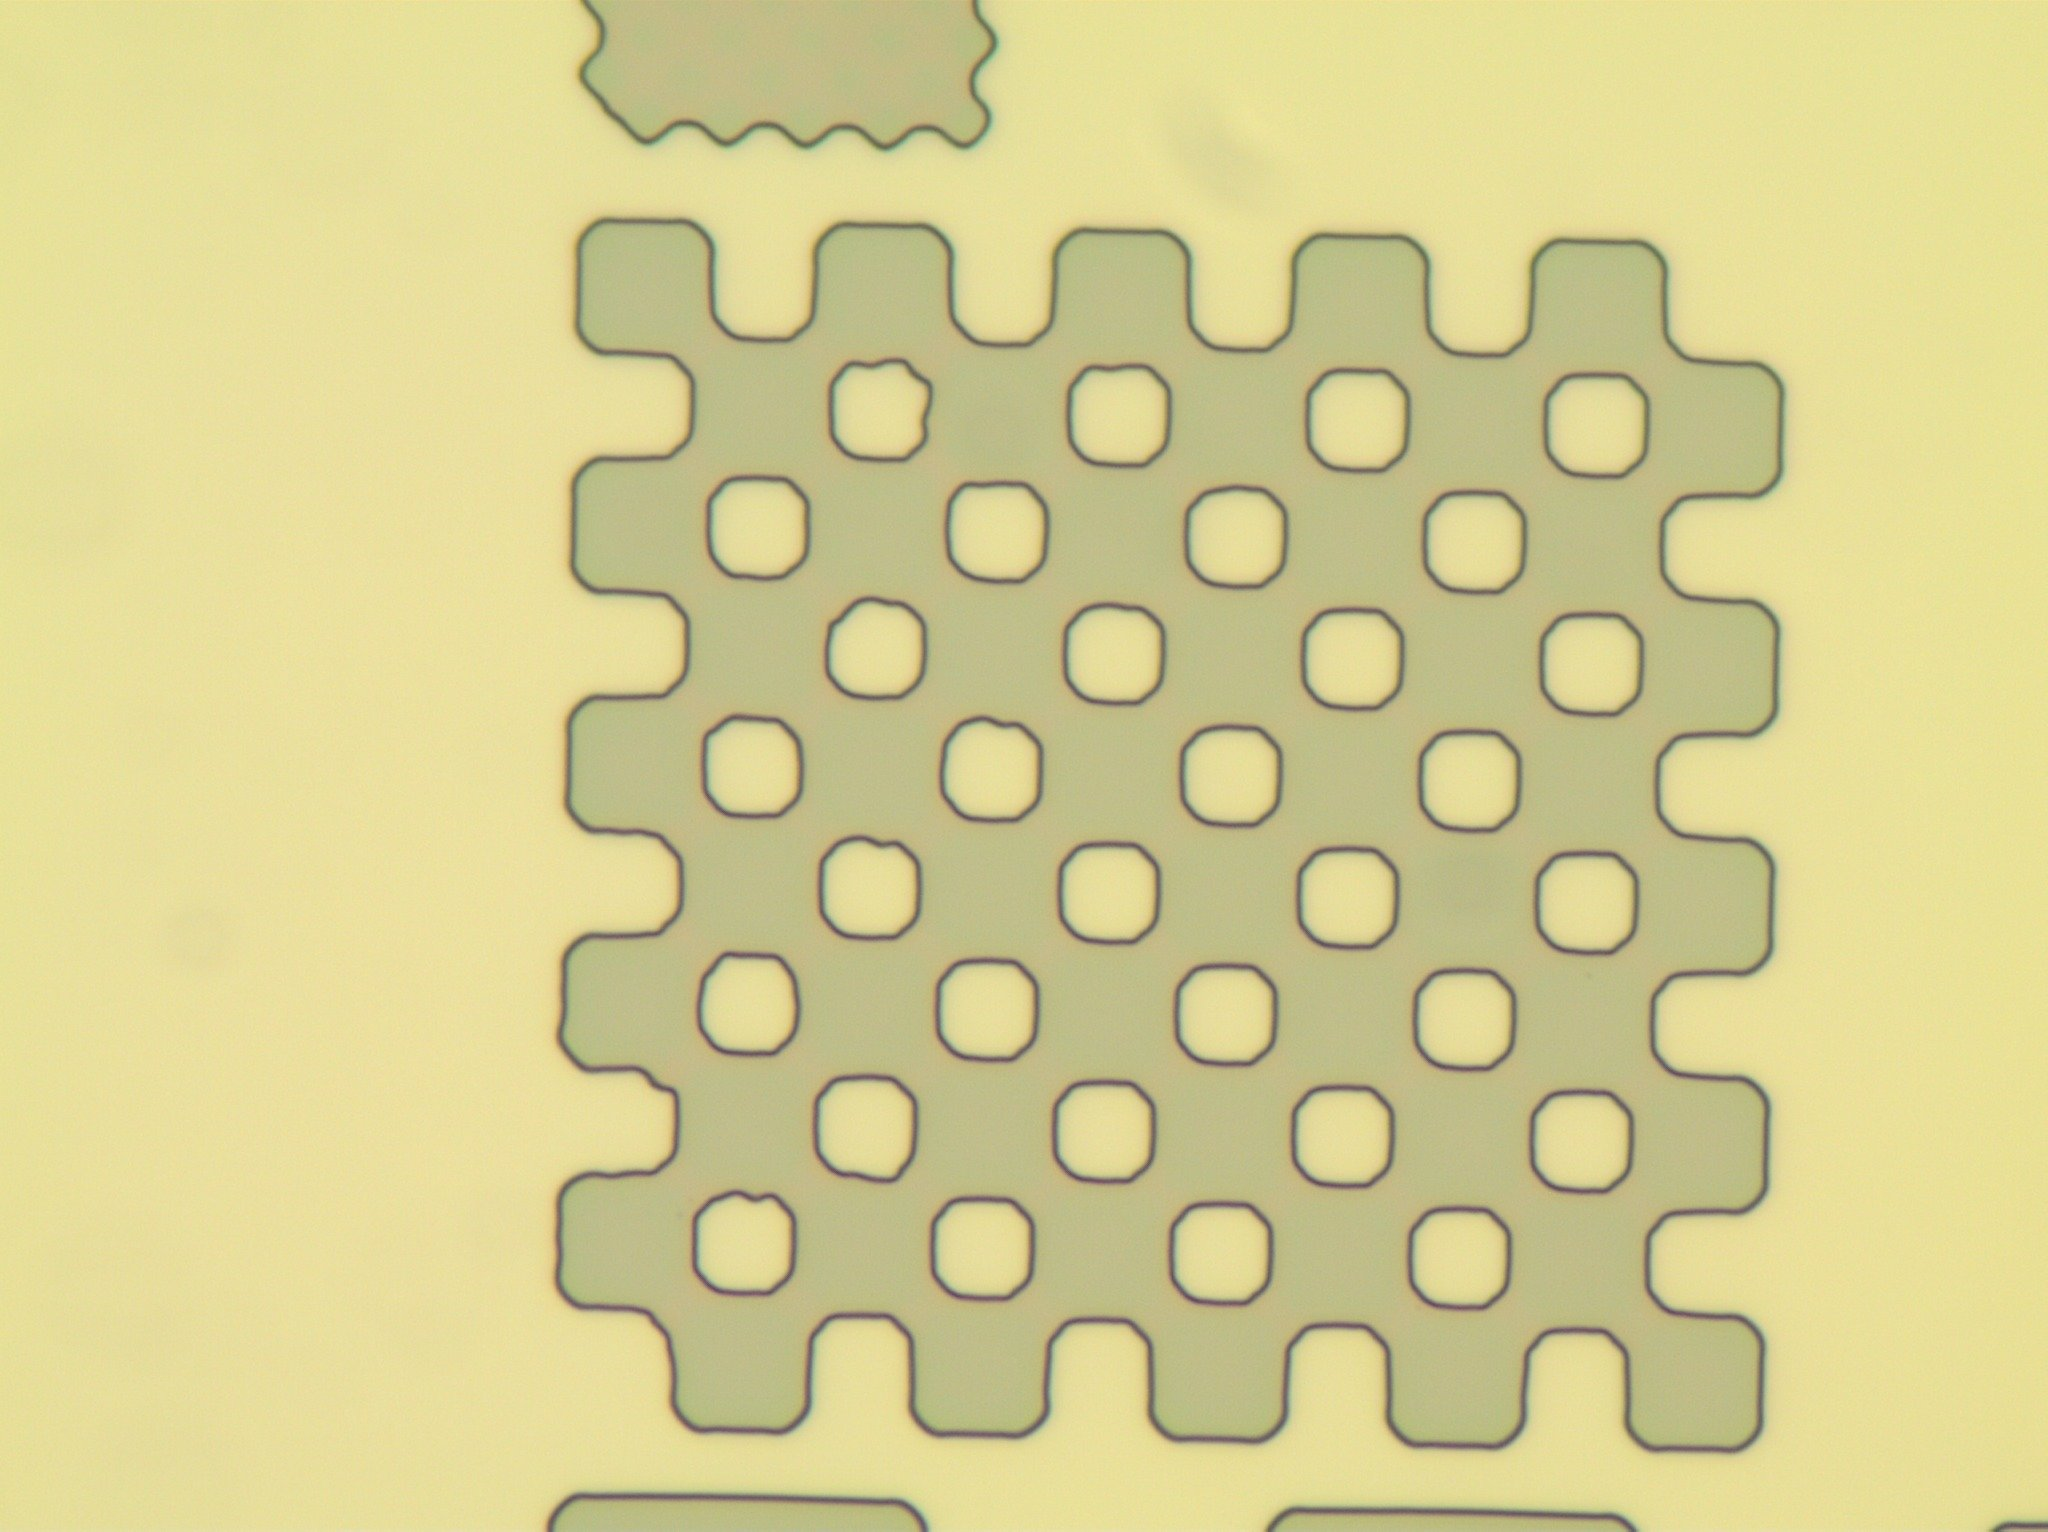
\includegraphics{data/b2d1.jpg}}
	\caption{Sample of the negative resist pattern with an exposure time of 0.5 minutes.Taking into account that a negative tone was used, it can be seen that the sample was clearly overexposed.}
	\label{fig:b2d1}
\end{figure}
\begin{figure}[H]
	\centering
	\resizebox{\linewidth}{!}{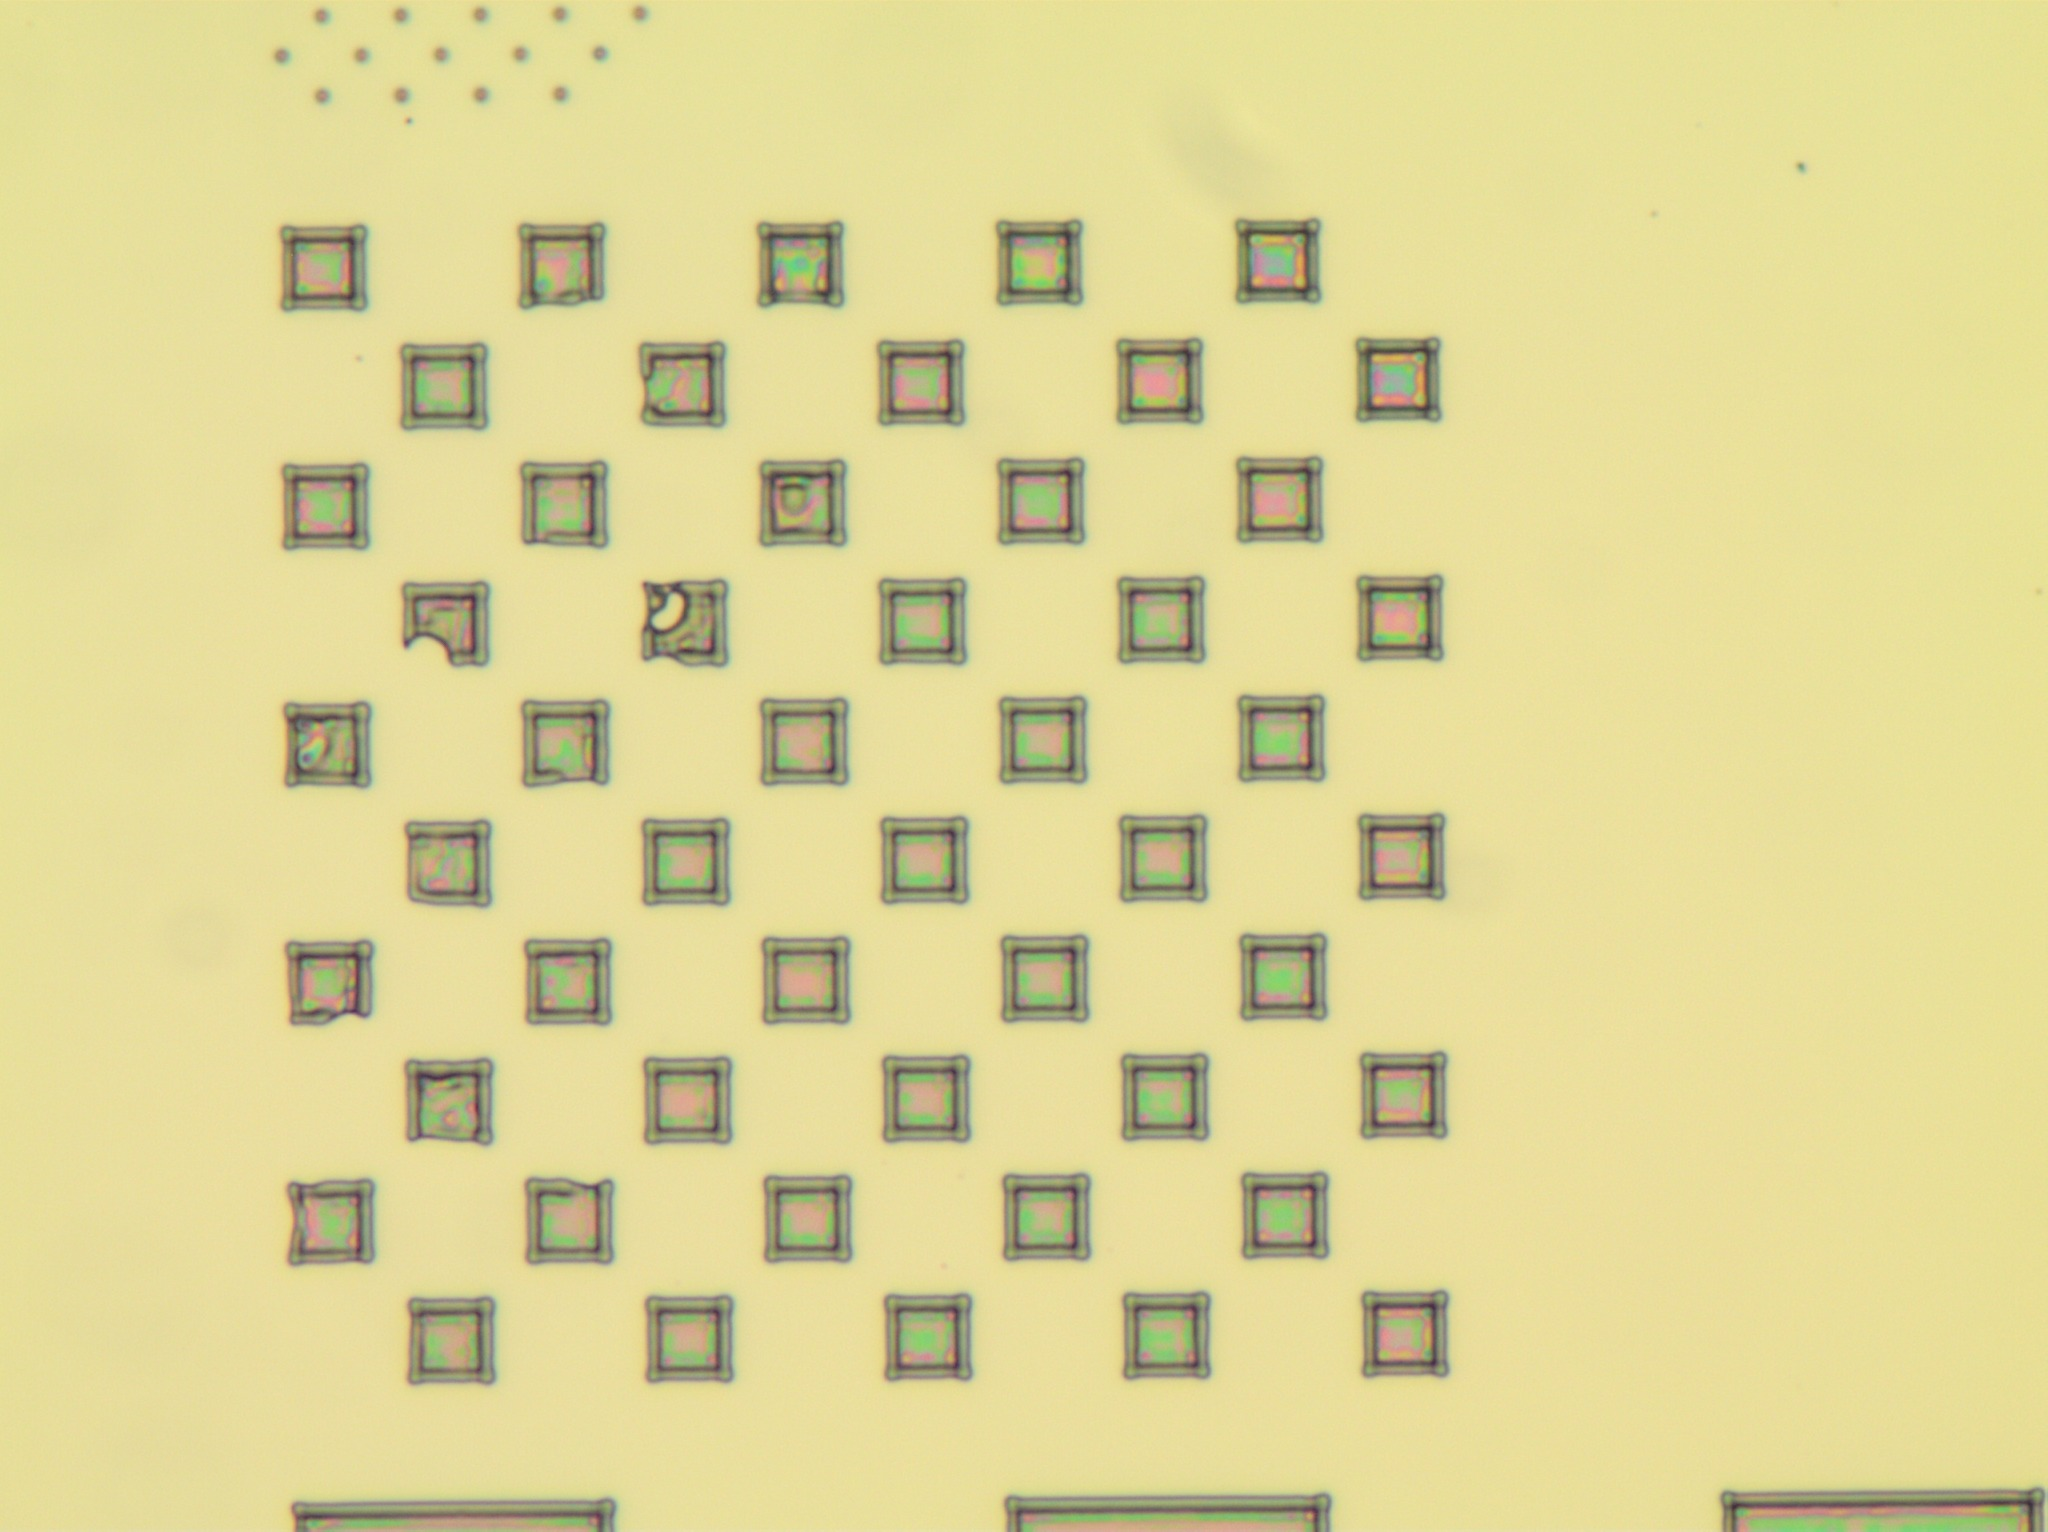
\includegraphics{data/b2h1.jpg}}
	\caption{Sample of the negative resist pattern with an exposure time of 0.2 minutes. Note that the sample is underexposed.}
	\label{fig:b2h1}
\end{figure}
\begin{figure}[H]
	\centering
	\resizebox{\linewidth}{!}{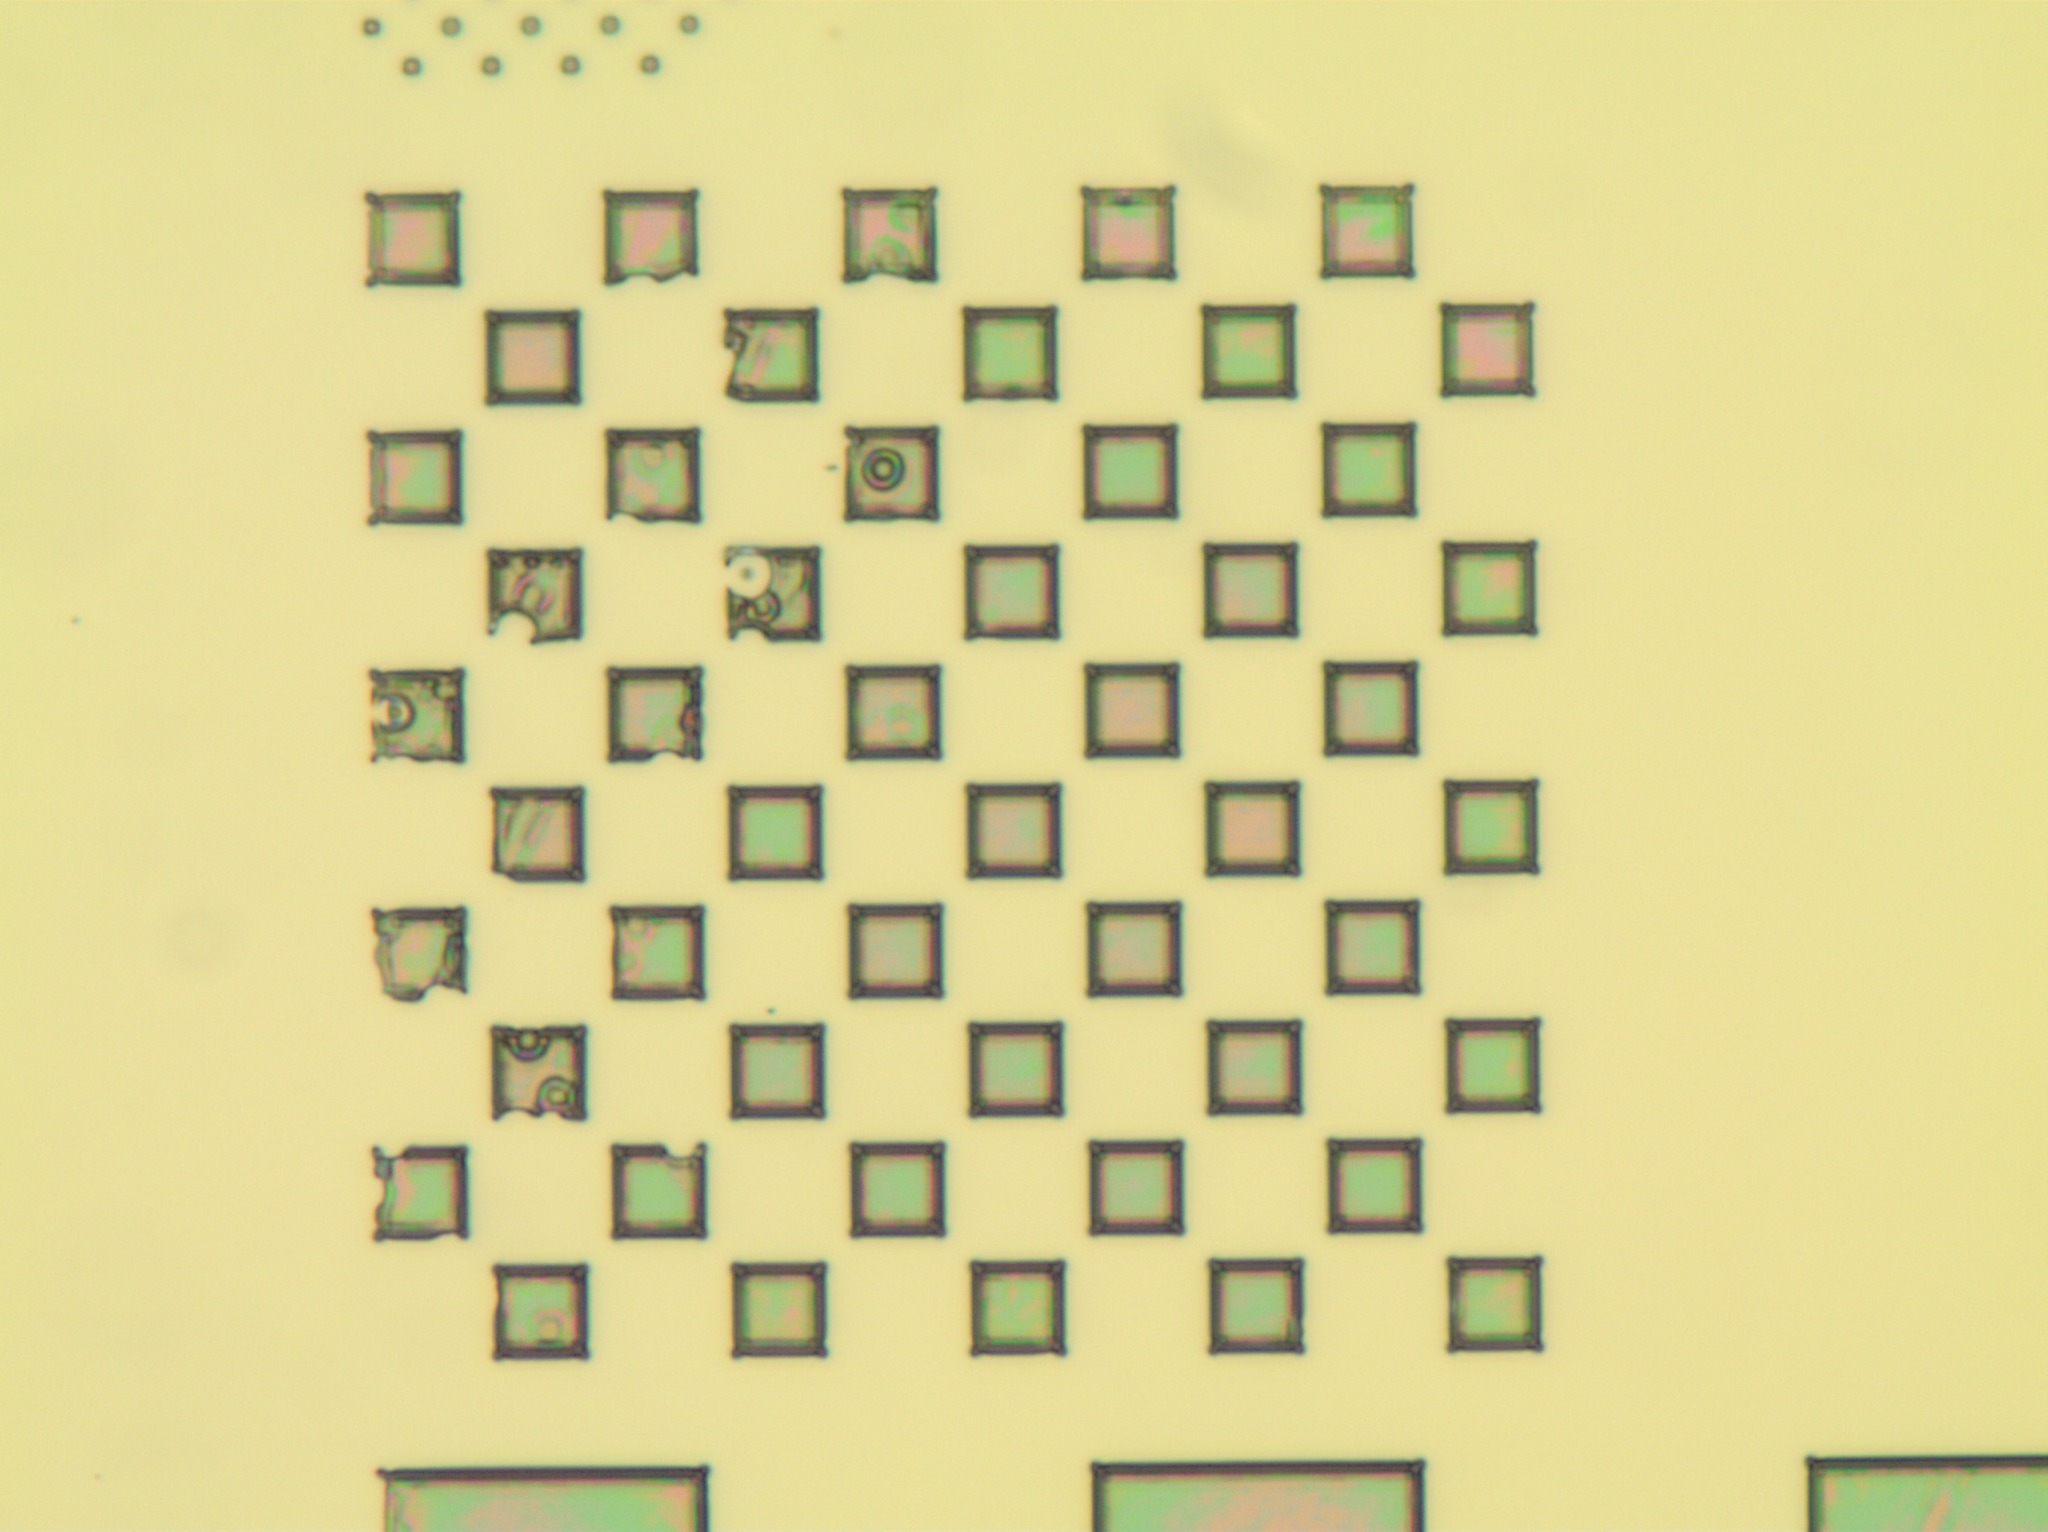
\includegraphics{data/b2i1.jpg}}
	\caption{Sample of the negative resist pattern with an exposure time of 0.3 minutes. The sample is again underexposed, but not as much as the sample with an exposure time of 0.2 minutes.}
	\label{fig:b2i1}
\end{figure}

From this we conclude that when using image reversal with the AZ5241 an exposure time of around 0.4 minutes will be optimal for lithography. Images of the checkerboard pattern of the sample with an exposure time of 0.5 minutes under the Hitachi S4800 SEM are seen below:


\begin{figure}[H]
	\centering
	\resizebox{\linewidth}{!}{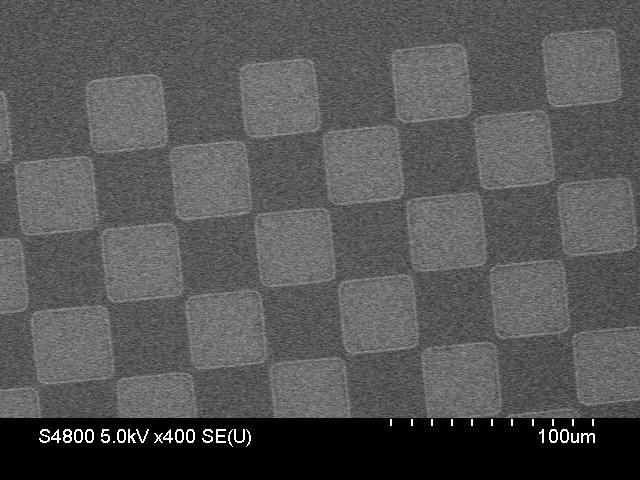
\includegraphics{data/sem/b2d26_q26.jpg}}
	\caption{SEM}
	\label{fig:b2d26_q26}
\end{figure}
\begin{figure}[H]
	\centering
	\resizebox{\linewidth}{!}{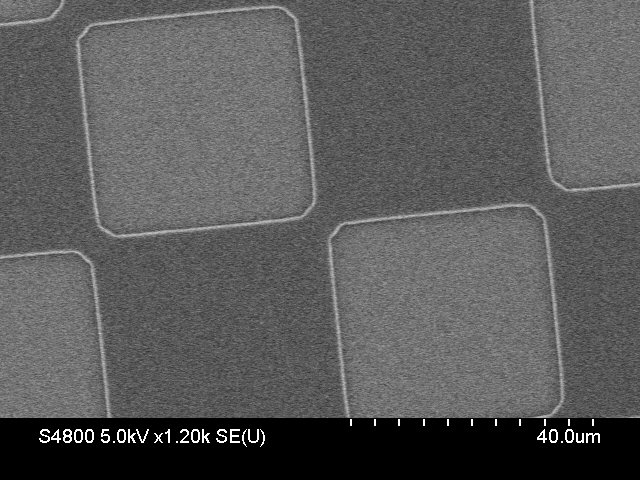
\includegraphics{data/sem/b2d27_q27.jpg}}
	\caption{SEM}
	\label{fig:b2d27_q27}
\end{figure}
\begin{figure}[H]
	\centering
	\resizebox{\linewidth}{!}{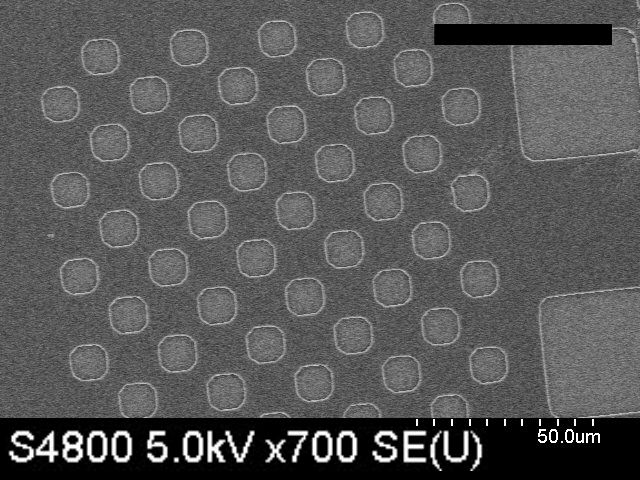
\includegraphics{data/sem/b2d28_q28.jpg}}
	\caption{SEM}
	\label{fig:b2d28_q28}
\end{figure}
\begin{figure}[H]
	\centering
	\resizebox{\linewidth}{!}{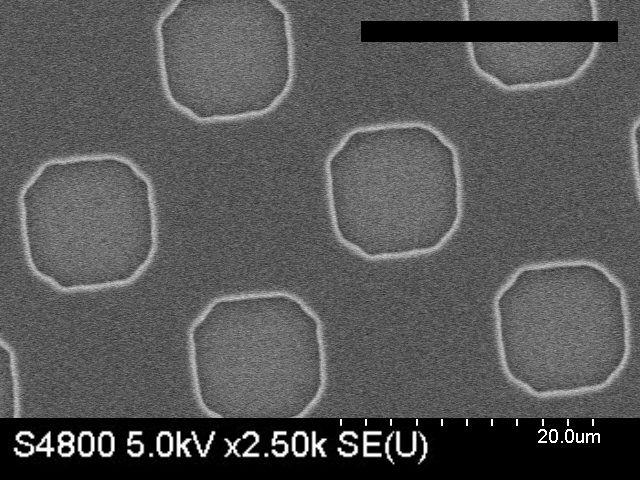
\includegraphics{data/sem/b2d29_q29.jpg}}
	\caption{SEM}
	\label{fig:b2d29_q29}
\end{figure}

\begin{table}[H]
    \centering
    \caption{Positive resist thickness}
    \begin{tabular}{X l l l}
        Sample & $\Delta h_1$ (nm)& $\Delta h_2$ (nm) \\ 
        \hline\hline
        b & 1608.1  &   1578.3  \\
        c & 1662.7  &   1676.4  \\
        d & 320.9   &   314.0   \\
        e & 1628.6  &   1628.6  \\
        f & 1587.7  &   1596.2  \\
        \hline
    \end{tabular}
    \label{tab:pos_profile}
\end{table}

\begin{table}[H]
    \centering
    \caption{Negative resist thickness}
    \begin{tabular}{X l l l}
        Sample & $\Delta h_1$ (nm) & $\Delta h_2 (nm)$ \\ 
        \hline\hline
        a & 1392.5  &   1376.4  \\
        b & 1416.9  &   1547.43 \\
        c & 1673.2  &   1690.1  \\
        d & 1551.7  &   1522.6  \\
        e & 1557.2  &   1547.1  \\
        f & 1552.0  &   1524.1  \\
        g & 45.047  &   ~       \\
        h & 801.17  &   926.17  \\
        i & 575.98  &   556.88  \\
        \hline
    \end{tabular}
    \label{tab:neg_profile}
\end{table}

It is clear from the table that the positive sample d and negative sample g almost had no activation of the photosensitive resist.

While the exposure time is of importance, the development time also plays a role. During the analyzing of a batch of positive resist samples, it was found that the quality of the samples fluctuated, and that in general longer exposure times were required. 
